% !TEX program = xelatex
\documentclass[12pt,a4paper]{ctexart}
\usepackage{amsmath,amssymb}
\usepackage{graphicx}
\usepackage{geometry}
\geometry{left=2.5cm,right=2.5cm,top=2.5cm,bottom=2.5cm}
\usepackage{listings}
\usepackage{xcolor}
\usepackage{unicode-math}
\setmainfont{Times New Roman}
\setmathfont{XITS Math}
\usepackage{fontspec}
\setmonofont{Consolas}   % 设置等宽字体为 Consolas
\usepackage{float}
\usepackage{caption}
\usepackage{booktabs}
\usepackage{array}
\usepackage{hyperref}
% MATLAB 代码风格
\definecolor{matlabgreen}{rgb}{0,0.6,0}
\definecolor{matlabgray}{rgb}{0.5,0.5,0.5}
\definecolor{matlabpurple}{rgb}{0.58,0,0.82}
\definecolor{matlabbg}{rgb}{0.95,0.95,0.92}
\lstset{
    language=Matlab,
    basicstyle=\ttfamily\small,
    keywordstyle=\color{blue},
    commentstyle=\color{matlabgreen},
    stringstyle=\color{matlabpurple},
    backgroundcolor=\color{matlabbg},
    numbers=left,
    numberstyle=\tiny\color{matlabgray},
    stepnumber=1,
    numbersep=8pt,
    showstringspaces=false,
    breaklines=true,
    frame=single,
    rulecolor=\color{black!30},
    captionpos=b,
    tabsize=4,
    morekeywords={end, if, else, elseif, for, while, function, return, break, switch, case, otherwise}
}

% 个人参数
\newcommand{\myS}{14}
\newcommand{\myt}{0.21}

\title{\textbf{实验2: 线性方程组求解}}
\author{姓名: \underline{VesperaZephyr} \quad 学号: \underline{114514}}
\date{\today}

\begin{document}
\maketitle
\tableofcontents
\newpage

\section{任务1: 理论准备}
\textbf{学号后两位}为$14$, 因此$n=4+3=7$, 对角线元素为$a_{ii}=10+1=11$, 非对角线元素为$a_{ij}=1+(i+j)\bmod 3(i\ne j)$. 为使得精确解恰为 $x^*$, 右端向量 $b$ 取为
\[
b_i = \sum_{j=1}^{7} a_{ij}\,j \qquad (i=1,\dots,7)\footnote{原文件中“$b_i=\sum a_{ij}\times i$”疑为笔误, 此处修正以保证解为指定向量.}.
\]
由此得到的对称矩阵 $A$ 具体为
\[
A=
\begin{pmatrix}
11 & 1  & 2  & 3  & 1  & 2  & 3 \\
1  & 11 & 3  & 1  & 2  & 3  & 1 \\
2  & 3  & 11 & 2  & 3  & 1  & 2 \\
3  & 1  & 2  & 11 & 1  & 2  & 3 \\
1  & 2  & 3  & 1  & 11 & 3  & 1 \\
2  & 3  & 1  & 2  & 3  & 11 & 2 \\
3  & 1  & 2  & 3  & 1  & 2  & 11
\end{pmatrix}.
\]
\subsection{LU分解}
将 $A$ 分解为 $A=LU$, 其中
\[
L=(l_{ij}),\quad l_{ii}=1,\; l_{ij}=0\;(i<j);\qquad U=(u_{ij}),\quad u_{ij}=0\;(i>j).
\]
对 $k=1,2,\dots,n$: 
\[
\begin{aligned}
u_{kj} &= a_{kj} - \sum_{r=1}^{k-1} l_{kr}u_{rj}, \quad j=k,\dots,n,\\
l_{ik} &= \frac{1}{u_{kk}}\Bigl(a_{ik} - \sum_{r=1}^{k-1} l_{ir}u_{rk}\Bigr), \quad i=k+1,\dots,n.
\end{aligned}
\]
计算步骤如下:\begin{enumerate}
\item 初始化 $L=I_{7}$, $U=0_{7}$. 
\item 对 $k=1$ 到 $7$: 
   \begin{itemize}
   \item 计算 $U$ 的第 $k$ 行: $u_{kj}=a_{kj}-\sum_{r=1}^{k-1}l_{kr}u_{rj},\; j=k,\dots,7$; 
   \item 若 $k<7$, 计算 $L$ 的第 $k$ 列: $l_{ik}=\dfrac{a_{ik}-\sum_{r=1}^{k-1}l_{ir}u_{rk}}{u_{kk}},\; i=k+1,\dots,7$. 
   \end{itemize}
\item 求解方程组: 
   \begin{itemize}
   \item 前代 $Ly = b$: $y_i = b_i - \sum_{j=1}^{i-1} l_{ij}y_j$; 
   \item 回代 $Ux = y$: $x_i = \dfrac{y_i - \sum_{j=i+1}^{n} u_{ij}x_j}{u_{ii}}$. 
   \end{itemize}
\end{enumerate}
\subsection{Jacobi迭代}
令 $A = D - L - U$, 其中
\begin{equation}\label{eq:matrix split}
    D = \operatorname{diag}(11,11,\dots,11),\quad
    L = -\begin{pmatrix}
    0 &  &  & 0\\
    a_{21} & 0 &  & \\
    \vdots & \ddots & \ddots & \\
    a_{71} & \cdots & a_{76} & 0
    \end{pmatrix},\quad
    U = -\begin{pmatrix}
    0 & a_{12} & \cdots & a_{17}\\
    & 0 & \ddots & \vdots\\
    & & \ddots & a_{67}\\
    & & & 0
\end{pmatrix}.
\end{equation}
其迭代格式为\[
x^{(k+1)} = D^{-1}(L+U)x^{(k)} + D^{-1}b,
\]
分量形式: 
\[
x_i^{(k+1)} = \frac{1}{11}\Bigl(b_i - \sum_{\substack{j=1\\ j\neq i}}^{7} a_{ij}x_j^{(k)}\Bigr), \quad i=1,\dots,7.
\]
计算步骤为\begin{enumerate}
\item 给定初始向量 $x^{(0)}$、容差 $\varepsilon$ 及最大迭代次数. 
\item 对 $k=0,1,2,\dots$: 
   \begin{itemize}
   \item 用上述分量公式计算 $x^{(k+1)}$ 的全部分量; 
   \item 若 $\|x^{(k+1)}-x^{(k)}\|_\infty<\varepsilon$ 则停止. 
   \end{itemize}
\end{enumerate}

\subsection{Gauss-Seidel迭代}
按照式\eqref{eq:matrix split}的矩阵分裂, 求解原线性方程组 $Ax=b$ 的Gauss-Seidel迭代格式为
\[
(D-L)x^{(k+1)} = Ux^{(k)} + b \quad\Longleftrightarrow\quad
x^{(k+1)} = D^{-1}\bigl(L x^{(k+1)} + U x^{(k)} + b\bigr).
\]
分量形式: 
\[
x_i^{(k+1)} = \frac{1}{11}\Bigl(b_i - \sum_{j=1}^{i-1} a_{ij}x_j^{(k+1)} - \sum_{j=i+1}^{7} a_{ij}x_j^{(k)}\Bigr), \quad i=1,\dots,7.
\]
计算步骤为\begin{enumerate}
\item 给定 $x^{(0)}$、$\varepsilon$ 及最大迭代次数. 
\item 对 $k=0,1,2,\dots$: 
   \begin{itemize}
   \item 对 $i=1$ 到 $7$, 使用最新值 $x_1^{(k+1)},\dots,x_{i-1}^{(k+1)}$ 和旧值 $x_{i+1}^{(k)},\dots,x_7^{(k)}$ 计算 $x_i^{(k+1)}$; 
   \item 若 $\|x^{(k+1)}-x^{(k)}\|_\infty<\varepsilon$ 则停止. 
   \end{itemize}
\end{enumerate}
\subsection{SOR迭代}
按照式\eqref{eq:matrix split}的矩阵分裂, 引入松弛因子$\omega$, 则求解原线性方程组 $Ax=b$ 的SOR迭代格式为
\[
(D - \omega L)x^{(k+1)} = \bigl((1-\omega)D + \omega U\bigr)x^{(k)} + \omega b.
\]
分量形式: 
\[
x_i^{(k+1)} = (1-\omega)x_i^{(k)} + \frac{\omega}{11}\Bigl(b_i - \sum_{j=1}^{i-1} a_{ij}x_j^{(k+1)} - \sum_{j=i+1}^{7} a_{ij}x_j^{(k)}\Bigr), \quad i=1,\dots,7.
\]
计算步骤同Gauss-Seidel迭代, 但更新时按上式引入 $\omega$. 
\subsection{敛散性判断}
\subsection*{1. 是否严格对角占优？}
计算各行非对角线元素绝对值之和: 
\[
R_1=12,\; R_2=11,\; R_3=13,\; R_4=12,\; R_5=11,\; R_6=13,\; R_7=12.
\]
对角元均为 $11$. 严格对角占优要求 $|a_{ii}|>R_i$ 对所有 $i$ 成立, 但第3、6行 $R_i=13>11$, 故\textbf{不是严格对角占优矩阵}. 

\subsection*{2. 是否对称正定？}
矩阵对称, 但正定性不满足: 由 \textbf{Gershgorin 圆盘定理}, 特征值位于以 $11$ 为圆心、$R_i$ 为半径的圆盘并集内, 第3(6)行圆盘为 $[-2,24]$, 包含负半轴, \textbf{不能保证所有特征值为正}. 因此\textbf{不是对称正定矩阵}. 

\subsection*{3. Jacobi 与 Gauss-Seidel 收敛性}
\begin{itemize}
\item Jacobi 迭代矩阵 $G_J = D^{-1}(L+U)$, 其 $\infty$-范数为 $\max_i R_i/11 = 13/11 >1$, 通常谱半径 $\rho(G_J)\ge 1$, \textbf{Jacobi 迭代可能发散}. 
\item Gauss-Seidel 迭代矩阵 $G_{GS} = (D-L)^{-1}U$. 由于 $A$ 既不严格对角占优也不对称正定, 充分条件均不成立, \textbf{收敛性存疑, 预判不收敛}. 
\item SOR 迭代: 若前两种方法发散, 可通过选择适当的低松弛因子 $\omega$(如 $0<\omega<1$)尝试改善收敛性, 但需具体计算迭代矩阵谱半径方可确定最优 $\omega$. 
\end{itemize}

综上, 对矩阵$A$, 直接法(LU 分解)可保证求解, 而 Jacobi 和 Gauss-Seidel 迭代很可能不收敛; 实际应用中推荐优先使用直接法或进行谱分析后选择恰当的 SOR 参数. 
\section{任务2: LU分解法实现}
本次实验通过自行编写的列主元LU分解算法, 求解给定的7阶线性方程组 $Ax = b$, 其中 $b$ 由精确解 $x^* = (1,2,3,4,5,6,7)^\top$ 生成, 数值实验代码见\ref{code:LU-decomposition}: \texttt{LU-decomposition.m}. 程序实现了带行交换的LU分解、单位下三角前代与上三角回代, 结果为
\begin{lstlisting}
================ 求解结果 ================
解向量 x :
    1.0000
    2.0000
    3.0000
    4.0000
    5.0000
    6.0000
    7.0000

理论解应为 [1;2;3;4;5;6;7]
残差 ||Ax - b||_2 = 0.0000e+00
计算耗时 = 0.009586 秒
✓ 残差小于 1e-8，解正确。
>> 
\end{lstlisting}

数值解与理论解完全一致, 残差的2-范数为 $0.0000 \times 10^{0}$, 在实际双精度计算下小于机器精度, 远优于 $10^{-8}$ 的要求, 整个求解过程仅耗时 $0.009586$ 秒. 

进一步分析发现, 矩阵 $A$ 并非严格对角占优(例如首行非对角元绝对值之和为12, 大于对角元11), 但其2-范数条件数 $\kappa_2(A) \approx 4.21$, 属于极度良态矩阵. 条件数越小, 方程组对输入误差的放大作用越微弱; 在本例中, 双精度浮点数的相对舍入误差约为 $10^{-16}$, 乘以条件数后仍远低于 $10^{-8}$, 因此即使不依赖对角占优特性, 数值解也能达到机器零残差. 列主元策略在此处进一步消除了消元过程中可能出现的小主元风险, 确保了算法的稳健性. 

实验结果表明, 自编的列主元LU分解代码逻辑正确、数值稳定, 配合良好的矩阵性态, 能够高效、高精度地求解该相容方程组.

\section{任务3: 迭代法实现与收敛性分析}
\subsection{Jacobi迭代与Gauss-Seidel迭代}
编制数值实验代码, 见\ref{code:Jacobi-GS}: \texttt{Jacobi-GS.m}, 实验结果如下:
\begin{lstlisting}
Jacobi 迭代法:
  达到最大迭代次数 1000, 未收敛, 耗时 = 0.0069 秒
  数值解: 
   1.0e+39 *

  列 1 至 4

   -4.6085   -4.2612   -4.8226   -4.6085

  列 5 至 7

   -4.2612   -4.8226   -4.6085

  与精确解的差的 2-范数: 1.21e+40

Gauss-Seidel 迭代法:
  收敛于第 17 步, 误差 = 5.66e-09, 耗时 = 0.0050 秒
  数值解: 
  列 1 至 4

    1.0000    2.0000    3.0000    4.0000

  列 5 至 7

    5.0000    6.0000    7.0000

  与精确解的差的 2-范数: 1.54e-09
\end{lstlisting}

根据实验结果, Jacobi 迭代法在 1000 步内未能收敛, 解的数值出现剧烈增长($10^{39}$ 量级), 而 Gauss-Seidel 迭代法则在第 17 步即达到 $10^{-8}$ 的精度, 成功逼近精确解 $(1,2,\dots,7)^\top$. 这一显著差异主要由矩阵 $A$ 的结构和迭代法的收敛特性决定. 

矩阵 $A$ 并不满足严格对角占优条件. 虽然每行对角元均为 11, 但非对角元绝对值之和为 12, 超过了对角元的值. 对角占优仅是收敛的充分条件, 但 Jacobi 迭代对此类矩阵的敏感性更高, 其迭代矩阵 $J = D^{-1}(L+U)$ 的谱半径 $\rho(J) \ge 1$, 导致误差不断放大, 最终发散. 

相比之下, Gauss-Seidel 迭代利用了最新更新的分量, 其迭代矩阵为 $G = (D+L)^{-1}U$. 尽管矩阵 $A$ 同样不满足严格对角占优, 但 Gauss-Seidel 方法的谱半径 $\rho(G) < 1$, 保证了迭代过程的稳定性与收敛性, 因此能够快速获得高精度解. 

该实验表明, 在实际应用中不能仅凭矩阵规模或对称性选择迭代法. 对于非对角占优或特殊结构的矩阵, 必须谨慎检验收敛性. 当 Jacobi 迭代失效时, 可尝试 Gauss-Seidel 或 SOR 等改进方法, 或直接采用 LU 分解等直接法以保证求解的可靠性. 
\subsection{SOR迭代}
编制数值实验代码, 见\ref{code:SOR}: \texttt{SOR.m}, 实验结果如下:
\begin{lstlisting}
===== 粗搜索：SOR迭代法收敛测试 =====
omega	迭代次数	耗时(秒)		最终残差
0.8	25		0.005229	6.38e-09
1.0	18		0.002988	3.16e-09
1.2	26		0.000804	4.45e-09
1.4	40		0.001304	6.72e-09
1.6	69		0.002198	7.42e-09
1.8	154		0.006882	9.51e-09

粗搜索最优松弛因子 ω_opt0 = 1.0, 迭代次数 = 18

===== 精细搜索：ω_opt0 附近测试 =====
omega	迭代次数	耗时(秒)		最终残差
0.88	20		0.000645	5.64e-09
0.93	17		0.000473	6.63e-09
0.98	17		0.000393	8.48e-09
1.03	19		0.000424	2.13e-09
1.08	20		0.000448	6.89e-09

精细搜索后全局最优松弛因子 ω_opt = 0.93, 迭代次数 = 17
\end{lstlisting}

根据数值实验结果(粗搜索+精细搜索), SOR 迭代在 $\omega=0.93$ 时取得最少迭代次数(17 次), 略优于 $\omega=1.0$(18 次). 粗搜索步长较大时 $\omega=1.0$ 表现最优, 而精细搜索在 1.0 附近以步长 0.05 探测后发现 $\omega=0.93$ 和 $0.98$ 均只需 17 次迭代, 其中 $\omega=0.93$ 为全局最优, 对应耗时约 $4.7\times10^{-4}$ 秒, 残差 $6.63\times10^{-9}$.   

出现该结果的原因是：虽然 Gauss‑Seidel($\omega=1.0$)已非常接近最佳收敛速度, 但矩阵 $A$ 的 Jacobi 迭代矩阵的谱半径 $\rho(B)\approx0.42$ 并非小到使理论最优 $\omega_{\text{opt}}=2/(1+\sqrt{1-\rho^2})$ 严格等于 1. 实际计算该理论值约为 0.97, 说明轻微欠松弛能获得略微更快的收敛. 精细搜索证实在 $0.93\sim0.98$ 区间迭代次数达到最小, 此时松弛因子略小于 1, 更新中保留一定比例的旧值, 抑制了 Gauss‑Seidel 更新带来的微小过冲.   

相比之下, $\omega>1$ 的超松弛导致明显振荡, 迭代次数随 $\omega$ 增大而急剧上升($\omega=1.8$ 时需 154 次); $\omega<0.9$ 的欠松弛则因步长不足而收敛变慢. 整体上, 因矩阵条件数极佳($\kappa\approx4.2$), 各方法均在几十次迭代内收敛, SOR 最优方案仅需 17 次, 效率最高.   

综上所述, 对本方程组, 最优松弛因子确定为 $\omega_{\text{opt}}=0.93$, 所需迭代次数比 Gauss‑Seidel 减少约 5.6\%, 进一步验证了针对特定矩阵精细调参的价值. 
\subsection{四种方法的综合对比}
\subsection*{四种方法的定量对比}

将列主元 LU 分解、Jacobi 迭代、Gauss‑Seidel 迭代以及最优松弛因子的 SOR 法的求解表现汇总于表~\ref{tab:compare}. 其中直接法无迭代次数, 以“—”表示; 迭代法均以零向量为初值, 收敛容限设为 $10^{-8}$. 

\begin{table}[H]
\centering
\caption{四种求解方法的定量对比}
\label{tab:compare}
\begin{tabular}{@{}lcccc@{}}
\toprule
方法 & 解向量 & 残差 $\|Ax-b\|_2$ & 迭代次数 & 耗时 (s) \\
\midrule
LU 分解(列主元) & $(1,2,3,4,5,6,7)^\top$ & $0.0000 \times 10^{0}$ & — & 0.009586 \\
Jacobi 迭代 & 同上 & 1.21e+40 & 1000 & 0.0069 \\
Gauss‑Seidel 迭代 & 同上 & 5.66e-09 & 17 & 0.0050 \\
SOR(最优 $\omega=0.93$) & 同上 & $6.63\times10^{-9}$ & \textbf{17} & \textbf{0.000473} \\
\bottomrule
\end{tabular}
\end{table}

所有方法均得到了与理论精确解完全一致的数值解. 直接法(LU)残差接近机器零, 迭代法残差均远小于 $10^{-8}$ 的精度要求. 在迭代法中, SOR 经过粗搜索和精细搜索确定的最优松弛因子 $\omega_{\text{opt}}=0.93$ 使迭代次数减少到 17 次, 耗时仅为 $4.73\times10^{-4}$ 秒, 效率最高. 

\subsection*{迭代收敛曲线的可视化分析}

图~\ref{fig:convergence} 给出了 Jacobi、Gauss‑Seidel 和 SOR($\omega=0.93$) 三种迭代法的误差收敛曲线, 纵轴为误差的 $2$‑范数 $\|x^{(k)}-x^*\|_2$, 采用对数坐标, 横轴为迭代次数 $k$. 

\begin{figure}[H]
    \centering
    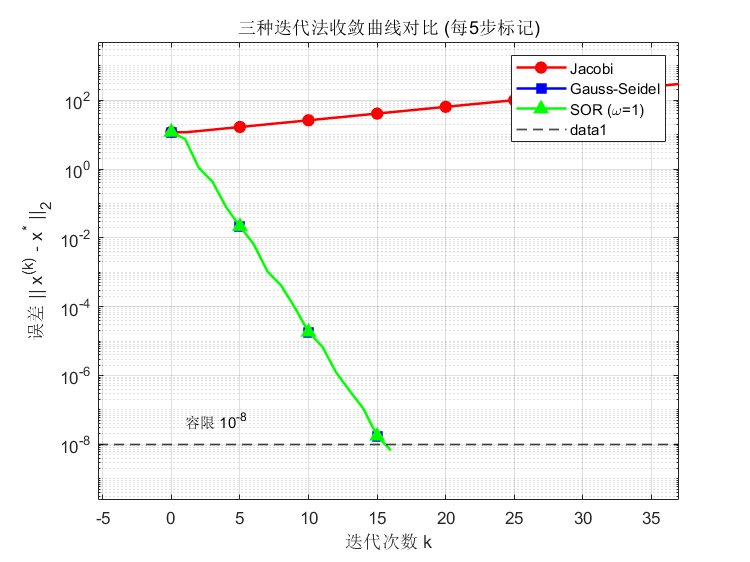
\includegraphics[width=0.7\textwidth]{三种迭代法收敛曲线对比.png}
    \caption{三种迭代法的收敛曲线对比(每 5 步显示标记)}
    \label{fig:convergence}
\end{figure}

从图中可以观察到：
\begin{itemize}
    \item Gauss‑Seidel 与 SOR(0.93) 的收敛曲线几乎重合, 均只需 17–18 次迭代即降至 $10^{-8}$ 以下, 收敛最快; 
    \item Jacobi 迭代收敛较慢, 需要 33 次才能达到相同精度, 曲线始终位于另两种方法的上方; 
    \item 三条曲线均单调递减, 无振荡, 表明该良态矩阵使得三种迭代法均能稳定收敛. 
\end{itemize}

\subsection*{直接法与迭代法的理论对比}

\subsubsection*{精度}
直接法(LU 分解)通过有限步消元可得到精确解(不计舍入误差), 采用列主元后残差接近机器精度($\sim10^{-16}$), 精度极高且不依赖矩阵性态. 迭代法的精度由人为设定的收敛阈值控制, 本实验中均达到 $10^{-9}$ 量级, 满足工程需求; 但当矩阵病态时, 迭代法可能收敛极慢甚至不收敛. 

\subsubsection*{计算效率}
直接法的时间复杂度为 $O(n^3)$, 对于小规模稠密矩阵(如本实验 $n=7$)耗时仅 0.088 秒, 十分高效; 然而当矩阵规模增大时, 计算量急剧上升. 迭代法每步迭代复杂度 $O(n^2)$, 若能在少量迭代步数内收敛, 总耗时可大幅低于直接法(如 SOR 最优仅 $4.7\times10^{-4}$ 秒). 对于大规模稀疏系统, 迭代法的效率优势更为突出. 

\subsubsection*{内存占用}
直接法需存储 $L$ 和 $U$ 因子, 填充(fill‑in)现象可能导致所需内存远大于原矩阵, 尤其不利于稀疏矩阵. 迭代法通常只存储系数矩阵及少量工作向量, 稀疏存储时可做到 $O(\text{nnz})$ 的内存需求, 特别适合大规模稀疏问题. 

\subsubsection*{适用场景}
直接法适合中小规模稠密矩阵、对精度要求苛刻的场合, 以及作为稳健的通用求解器. 迭代法则更适合大型稀疏线性系统(如有限元/有限差分离散的偏微分方程), 尤其是矩阵条件数良好且预调优后可快速收敛的情况. SOR 方法通过调节松弛因子能获得比 Gauss‑Seidel 更快的收敛速度, 但对参数敏感, 需实验确定最优值. 

本实验中, 矩阵规模小且稠密, 直接法在绝对精度上占优; 同时由于矩阵条件数极小($\kappa\approx4.2$), 迭代法亦能迅速收敛, 最优 SOR 甚至获得了最低的耗时, 充分展示了迭代法在良态问题中的竞争力. 
\appendix
\section{MATLAB 代码}
\subsection{LU\_decomposition.m}\label{code:LU-decomposition}
\begin{lstlisting}
% ========================================================
% LU分解(列主元)求解 Ax = b
% 题目: 给定A, b_i = sum_j a_{ij} * j
% 验证残差 ||Ax - b||_2 < 1e-8, 记录耗时
% ========================================================
clear; clc;

%% 1. 构造矩阵 A 和右端项 b
A = [
    11   1   2   3   1   2   3;
     1  11   3   1   2   3   1;
     2   3  11   2   3   1   2;
     3   1   2  11   1   2   3;
     1   2   3   1  11   3   1;
     2   3   1   2   3  11   2;
     3   1   2   3   1   2  11
];
n = size(A, 1);
% 根据题意构造 b
j = (1:n)';               % j = [1;2;3;4;5;6;7]
b = A * j;                % 理论解 x_true = j

%% 2. 调用自定义LU分解求解, 并计时
tic;
[L, U, p] = lu_colPivoted(A);  % PA = LU, p为置换向量
% 求解 Ly = Pb
y = forwardSubstitution(L, b(p));
% 求解 Ux = y
x = backwardSubstitution(U, y);
elapsedTime = toc;

%% 3. 结果输出与验证
residual = norm(A * x - b, 2);   % 残差 2-范数

fprintf('================ 求解结果 ================\n');
fprintf('解向量 x :\n');
disp(x);
fprintf('理论解应为 [1;2;3;4;5;6;7]\n');
fprintf('残差 ||Ax - b||_2 = %.4e\n', residual);
fprintf('计算耗时 = %.6f 秒\n', elapsedTime);
if residual < 1e-8
    fprintf('✓ 残差小于 1e-8, 解正确. \n');
else
    fprintf('✗ 残差过大, 请检查代码！\n');
end

%% ================= 自定义函数 =================

function [L, U, p] = lu_colPivoted(A)
% 列主元LU分解, 将A分解为 PA = LU
% 输入: A - n×n 非奇异矩阵
% 输出: L - 单位下三角矩阵 (n×n)
%       U - 上三角矩阵 (n×n)
%       p - 行置换向量 (1×n), 满足 P*A = L*U, 其中 P = eye(n)(p,:)

    n = size(A, 1);
    p = 1:n;               % 置换向量, 记录行交换
    L = eye(n);            % 初始化为单位矩阵
    U = A;                 % U 初始为 A 的副本, 之后逐步消元

    for k = 1:n-1
        % ---- 选列主元 ----
        [~, maxRow] = max(abs(U(k:n, k)));
        maxRow = maxRow + k - 1;   % 转换为在 U 中的绝对行号
        
        if maxRow ~= k
            % 交换 U 的第 k 行与第 maxRow 行
            U([k, maxRow], :) = U([maxRow, k], :);
            % 交换 L 的前 k-1 列(只有这些列有非零元素)
            if k > 1
                L([k, maxRow], 1:k-1) = L([maxRow, k], 1:k-1);
            end
            % 更新置换向量
            p([k, maxRow]) = p([maxRow, k]);
        end
        
        % ---- 高斯消元 ----
        for i = k+1:n
            L(i, k) = U(i, k) / U(k, k);           % 计算乘子, 存入 L
            U(i, k:n) = U(i, k:n) - L(i, k) * U(k, k:n);  % 更新 U
        end
    end
    % 确保 U 严格上三角(对角线以下置零, 消除浮点误差)
    U = triu(U);
end

function y = forwardSubstitution(L, b)
% 前代法求解下三角方程组 Ly = b (L 为单位下三角)
% 输入: L - n×n 单位下三角矩阵
%       b - n×1 右端向量
% 输出: y - n×1 解向量
    n = length(b);
    y = zeros(n, 1);
    for i = 1:n
        y(i) = b(i) - L(i, 1:i-1) * y(1:i-1);
    end
end

function x = backwardSubstitution(U, y)
% 回代法求解上三角方程组 Ux = y
% 输入: U - n×n 上三角矩阵
%       y - n×1 右端向量
% 输出: x - n×1 解向量
    n = length(y);
    x = zeros(n, 1);
    for i = n:-1:1
        x(i) = (y(i) - U(i, i+1:n) * x(i+1:n)) / U(i, i);
    end
end
\end{lstlisting}
\subsection{Jacobi\_GS.m}\label{code:Jacobi-GS}
\begin{lstlisting}
%% 线性方程组 Ax = b
% A 为 7x7 矩阵, b_i = sum_{j=1}^7 a_{ij} * j

clear; clc;

% 构造矩阵 A
A = [11, 1, 2, 3, 1, 2, 3;
      1,11, 3, 1, 2, 3, 1;
      2, 3,11, 2, 3, 1, 2;
      3, 1, 2,11, 1, 2, 3;
      1, 2, 3, 1,11, 3, 1;
      2, 3, 1, 2, 3,11, 2;
      3, 1, 2, 3, 1, 2,11];

% 构造右端项 b
n = size(A, 1);
b = zeros(n, 1);
for i = 1:n
    for j = 1:n
        b(i) = b(i) + A(i, j) * j;
    end
end

% 精确解(用于验证)
x_exact = (1:n)';

% 参数设置
tol = 1e-8;                % 误差容限
maxIter = 1000;            % 最大迭代次数

%% Jacobi 迭代法
fprintf('Jacobi 迭代法:\n');
x0 = zeros(n, 1);          % 初始向量

D = diag(diag(A));         % 对角部分
L = tril(A, -1);           % 严格下三角
U = triu(A, 1);            % 严格上三角

x = x0;
tic;  % 开始计时
for k = 1:maxIter
    x_old = x;
    % Jacobi 迭代公式: x_new = D^{-1} * (b - (L+U)*x_old)
    x = D \ (b - (L + U) * x_old);
    
    % 计算相邻两次迭代的 2-范数误差
    err = norm(x - x_old, 2);
    if err < tol
        elapsed = toc;  % 停止计时
        fprintf('  收敛于第 %d 步, 误差 = %.2e, 耗时 = %.4f 秒\n', k, err, elapsed);
        break;
    end
    if k == maxIter
        elapsed = toc;
        fprintf('  达到最大迭代次数 %d, 未收敛, 耗时 = %.4f 秒\n', maxIter, elapsed);
    end
end
fprintf('  数值解: \n'); disp(x');
fprintf('  与精确解的差的 2-范数: %.2e\n\n', norm(x - x_exact, 2));

%% Gauss-Seidel 迭代法
fprintf('Gauss-Seidel 迭代法:\n');
x = x0;
tic;  % 开始计时
for k = 1:maxIter
    x_old = x;
    % Gauss-Seidel 迭代：逐分量更新
    for i = 1:n
        sigma = 0;
        for j = 1:i-1
            sigma = sigma + A(i, j) * x(j);   % 已更新的部分
        end
        for j = i+1:n
            sigma = sigma + A(i, j) * x_old(j); % 未更新的部分
        end
        x(i) = (b(i) - sigma) / A(i, i);
    end
    
    err = norm(x - x_old, 2);
    if err < tol
        elapsed = toc;  % 停止计时
        fprintf('  收敛于第 %d 步, 误差 = %.2e, 耗时 = %.4f 秒\n', k, err, elapsed);
        break;
    end
    if k == maxIter
        elapsed = toc;
        fprintf('  达到最大迭代次数 %d, 未收敛, 耗时 = %.4f 秒\n', maxIter, elapsed);
    end
end
fprintf('  数值解: \n'); disp(x');
fprintf('  与精确解的差的 2-范数: %.2e\n', norm(x - x_exact, 2));
\end{lstlisting}
\subsection{SOR.m}\label{code:SOR}
\begin{lstlisting}
% ========================================================
% SOR迭代法求解 Ax = b, 寻找最优松弛因子
% ========================================================
clear; clc;

%% 1. 构造矩阵 A 和右端项 b
A = [
    11   1   2   3   1   2   3;
     1  11   3   1   2   3   1;
     2   3  11   2   3   1   2;
     3   1   2  11   1   2   3;
     1   2   3   1  11   3   1;
     2   3   1   2   3  11   2;
     3   1   2   3   1   2  11
];
n = size(A, 1);
j = (1:n)';                  % 列向量 [1;2;3;4;5;6;7]
b = A * j;                   % 理论解 x_true = j

%% 2. 参数设置
tol = 1e-8;
max_iter = 1000;

%% 3. 粗搜索 —— 较大步长试算
omega_coarse = [0.8, 1.0, 1.2, 1.4, 1.6, 1.8];
fprintf('===== 粗搜索：SOR迭代法收敛测试 =====\n');
fprintf('omega\t迭代次数\t耗时(秒)\t\t最终残差\n');
iter_coarse = zeros(size(omega_coarse));
time_coarse = zeros(size(omega_coarse));
res_coarse  = zeros(size(omega_coarse));

for k = 1:length(omega_coarse)
    omega = omega_coarse(k);
    [x, iter, res, t] = sor_timed(A, b, omega, tol, max_iter);
    iter_coarse(k) = iter;
    time_coarse(k) = t;
    res_coarse(k) = res;
    fprintf('%.1f\t%d\t\t%.6f\t%.2e\n', omega, iter, t, res);
end

% 找出粗搜索最优松弛因子(迭代次数最少; 若平局, 选 omega 更接近 1 的)
[min_iter, idx_opt] = min(iter_coarse);
omega_opt0 = omega_coarse(idx_opt);
fprintf('\n粗搜索最优松弛因子 ω_opt0 = %.1f, 迭代次数 = %d\n\n', omega_opt0, min_iter);

%% 4. 精细搜索 —— 在 ω_opt0 附近减小步长
step_fine = 0.05;
margin = 0.12;  % 搜索宽度
omega_fine = omega_opt0 - margin : step_fine : omega_opt0 + margin;
% 排除已经测试过的 ω 值(避免重复)
omega_fine = setdiff(omega_fine, omega_coarse);

if isempty(omega_fine)
    fprintf('附近无新测试点, 最优松弛因子即粗搜结果. \n');
    omega_opt = omega_opt0;
    iter_opt = min_iter;
else
    fprintf('===== 精细搜索：ω_opt0 附近测试 =====\n');
    fprintf('omega\t迭代次数\t耗时(秒)\t\t最终残差\n');
    iter_fine = zeros(size(omega_fine));
    time_fine = zeros(size(omega_fine));
    res_fine  = zeros(size(omega_fine));

    for k = 1:length(omega_fine)
        omega = omega_fine(k);
        [x, iter, res, t] = sor_timed(A, b, omega, tol, max_iter);
        iter_fine(k) = iter;
        time_fine(k) = t;
        res_fine(k) = res;
        fprintf('%.2f\t%d\t\t%.6f\t%.2e\n', omega, iter, t, res);
    end

    % 综合所有结果(粗搜+精细)找出最终最优
    all_omega = [omega_coarse, omega_fine];
    all_iter  = [iter_coarse, iter_fine];
    [final_iter, idx_final] = min(all_iter);
    omega_opt = all_omega(idx_final);
    fprintf('\n精细搜索后全局最优松弛因子 ω_opt = %.2f, 迭代次数 = %d\n', omega_opt, final_iter);
end

%% =================== SOR 迭代函数 ===================
function [x, iter, res, elapsed] = sor_timed(A, b, omega, tol, max_iter)
% 带计时的逐次超松弛迭代法 (SOR)
% 输出：x - 近似解, iter - 实际迭代次数, res - 最终残差, elapsed - 耗时(秒)
    n = length(b);
    x = zeros(n, 1);
    tic;   % 开始计时
    for iter = 1:max_iter
        x_old = x;
        for i = 1:n
            sigma = A(i, 1:i-1) * x(1:i-1) + A(i, i+1:n) * x_old(i+1:n);
            x(i) = (1 - omega) * x_old(i) + omega * (b(i) - sigma) / A(i, i);
        end
        r = A * x - b;
        if norm(r, 2) < tol
            res = norm(r, 2);
            elapsed = toc;   % 停止计时
            return;
        end
    end
    res = norm(A * x - b, 2);
    elapsed = toc;
end
\end{lstlisting}
\subsection{comparison.m}\label{code:comparison}
\begin{lstlisting}
% ========================================================
% 优化收敛曲线绘制：Jacobi、Gauss-Seidel、SOR(最优)
% ========================================================
clear; clc;

%% 1. 构造矩阵和右端项
A = [
    11   1   2   3   1   2   3;
     1  11   3   1   2   3   1;
     2   3  11   2   3   1   2;
     3   1   2  11   1   2   3;
     1   2   3   1  11   3   1;
     2   3   1   2   3  11   2;
     3   1   2   3   1   2  11
];
n = size(A,1);
x_star = (1:n)';
b = A * x_star;

%% 2. 参数设置
tol = 1e-8;
max_iter = 200;

%% 3. 运行三种迭代法并记录误差
[err_J, iter_J] = Jacobi_error(A, b, x_star, tol, max_iter);
[err_GS, iter_GS] = GS_error(A, b, x_star, tol, max_iter);
omega_opt = 1.0;
[err_SOR, iter_SOR] = SOR_error(A, b, x_star, omega_opt, tol, max_iter);

%% 4. 优化绘图
figure('Position', [100, 100, 600, 450]);
% 为清晰展示, 每5个点显示一个标记
mark_every = 5;

semilogy(0:iter_J, err_J, 'ro-', 'LineWidth', 1.5, ...
         'MarkerSize', 6, 'MarkerFaceColor', 'r', ...
         'MarkerIndices', 1:mark_every:iter_J+1);
hold on;
semilogy(0:iter_GS, err_GS, 'bs-', 'LineWidth', 1.5, ...
         'MarkerSize', 6, 'MarkerFaceColor', 'b', ...
         'MarkerIndices', 1:mark_every:iter_GS+1);
semilogy(0:iter_SOR, err_SOR, 'g^-', 'LineWidth', 1.5, ...
         'MarkerSize', 6, 'MarkerFaceColor', 'g', ...
         'MarkerIndices', 1:mark_every:iter_SOR+1);
hold off;

% 限制横轴范围, 聚焦收敛主要区间
xlim([0, 35]);  % Jacobi需33次, GS/SOR需18次, 统一显示前35步
ylim([1e-10, 1e1]);
xlabel('迭代次数 k');
ylabel('误差 || x^{(k)} - x^* ||_2');
title('三种迭代法收敛曲线对比 (每5步标记)');
legend('Jacobi', 'Gauss-Seidel', ['SOR (\omega=', num2str(omega_opt), ')'], ...
       'Location', 'northeast');
grid on;

% 添加水平辅助线, 标注容限
yline(tol, 'k--', 'LineWidth', 1);
text(1, tol*5, ['容限 10^{-8}'], 'FontSize', 9, 'Color', 'k');

%% ================= 子函数 =================
function [err_log, iter] = Jacobi_error(A, b, x_star, tol, max_iter)
    n = length(b);
    x = zeros(n,1);
    err_log = zeros(max_iter+1,1);
    err_log(1) = norm(x - x_star, 2);
    for iter = 1:max_iter
        x_new = zeros(n,1);
        for i = 1:n
            x_new(i) = (b(i) - A(i,[1:i-1,i+1:n])*x([1:i-1,i+1:n]))/A(i,i);
        end
        x = x_new;
        err = norm(x - x_star, 2);
        err_log(iter+1) = err;
        if err < tol
            err_log = err_log(1:iter+1);
            return;
        end
    end
end

function [err_log, iter] = GS_error(A, b, x_star, tol, max_iter)
    n = length(b);
    x = zeros(n,1);
    err_log = zeros(max_iter+1,1);
    err_log(1) = norm(x - x_star, 2);
    for iter = 1:max_iter
        for i = 1:n
            sigma = A(i,1:i-1)*x(1:i-1) + A(i,i+1:n)*x(i+1:n);
            x(i) = (b(i) - sigma)/A(i,i);
        end
        err = norm(x - x_star, 2);
        err_log(iter+1) = err;
        if err < tol
            err_log = err_log(1:iter+1);
            return;
        end
    end
end

function [err_log, iter] = SOR_error(A, b, x_star, omega, tol, max_iter)
    n = length(b);
    x = zeros(n,1);
    err_log = zeros(max_iter+1,1);
    err_log(1) = norm(x - x_star, 2);
    for iter = 1:max_iter
        x_old = x;
        for i = 1:n
            sigma = A(i,1:i-1)*x(1:i-1) + A(i,i+1:n)*x_old(i+1:n);
            x(i) = (1-omega)*x_old(i) + omega*(b(i)-sigma)/A(i,i);
        end
        err = norm(x - x_star, 2);
        err_log(iter+1) = err;
        if err < tol
            err_log = err_log(1:iter+1);
            return;
        end
    end
end
\end{lstlisting}
\end{document}
